\documentclass[english,a4paper,12pt]{report}
\usepackage{fancyhdr}
\usepackage{comment}
\usepackage{iftex}
\usepackage{longtable}
\usepackage{graphicx}
\usepackage{makecell}
\usepackage{geometry}
\usepackage{booktabs}
\usepackage{enumerate}
\usepackage{tabularx}
\usepackage{amsfonts}
\usepackage{blindtext}
\usepackage{qtree}
\usepackage{multicol}
\usepackage{amsmath,bm}
\usepackage{float}
\usepackage{amssymb}
\usepackage{wrapfig}
\restylefloat{figure}
\newcommand{\tabitem}{~~\llap{\textbullet}~~}
\usepackage{minted}
\usepackage{listings}
% \lstset{
%  basicstyle=\footnotesize,
%  language={[Objective]Caml},
%  breaklines=true,
%  tabsize=2,
%  frame=single,
%  numbers=left,
%  title=\lstname,
%  commentstyle=\color{mygreen},
%  numberstyle=\small\color{mygray},
%  stringstyle=\color{mymauve},
%  showstringspaces=false,
%  rulecolor=\color{black}
% }

\usepackage{xcolor}
\definecolor{codegreen}{rgb}{0,0.6,0}
\definecolor{codegray}{rgb}{0.5,0.5,0.5}
\definecolor{codepurple}{rgb}{0.58,0,0.82}
\definecolor{backcolour}{rgb}{0.95,0.95,0.92}
%Code listing style named "mystyle"

\usepackage{color}
\usepackage[draft=false]{hyperref}
\hypersetup{
    colorlinks=true, % make the links colored
    linkcolor=blue, % color TOC links in blue
    urlcolor=blue, % color URLs in blue
    linktoc=all % 'all' will create links for everything in the TOC
}
    
\urlstyle{same}
\lstdefinestyle{mystyle}{
  backgroundcolor=\color{backcolour},   commentstyle=\color{codegreen},
  keywordstyle=\color{magenta},
  numberstyle=\tiny\color{codegray},
  stringstyle=\color{codepurple},
  basicstyle=\ttfamily\footnotesize,
  breakatwhitespace=false,         
  breaklines=true,                 
  captionpos=b,     
  upquote=true,
  keepspaces=true,                 
  numbers=left,                    
  numbersep=5pt,                  
  showspaces=false,                
  showstringspaces=false,
  showtabs=false,                  
  tabsize=2
}


%"mystyle" code listing set
\lstset{style=mystyle}
\geometry{verbose,tmargin=4.5cm,bmargin=4cm,lmargin=1.5cm,rmargin=1cm,headheight=2.7cm,headsep=1.5cm,footskip=2cm}
\usepackage{array}
%
\def \hsp {\hspace{3mm}}
%
\makeatletter
\providecommand{\tabularnewline}{\\}
\makeatother
%
\ifxetex
\usepackage[T1]{fontenc}
\usepackage{fontspec}
\newfontfamily\nakulafont[AutoFakeBold=2]{Nakula}
\newfontfamily\liberationfont{Liberation Sans Narrow}
\newfontfamily\liberationsansfont{Liberation Sans}
\fi
%
\usepackage{tikz}
\usepackage{xcolor}
\usepackage{makecell}
%
% 
\definecolor{circleorange}{rgb}{1,0.17,0.08}
\definecolor{darkorange}{rgb}{1,0.27,0.1}
\definecolor{orange2}{rgb}{1,0.5,0.15}
\definecolor{orange3}{rgb}{1,0.65,0.25}
\definecolor{yellow1}{rgb}{0.95,0.77,0.2}
\newcommand{\Omit}[1]{}
\fancypagestyle{plain}{
  \fancyhead[LO]
  {
\textbf{CS4443 - Software Engineering} \newline 
\textbf {Indian Institute of Technology Hyderabad \newline
System Requirement Specification\newline
Group: H16 \newline}}
	  
%
	  \fancyhf[ROH]{

\begin{tikzpicture}[scale=0.25,every node/.style={transform shape}]
\draw [fill=circleorange,circleorange] (5,10) circle (1.15); 
\fill [darkorange] (5.06,8) -- (5.06,2) -- (7.3,1.2) -- (7.3,8.8) -- (5.06,8);
\fill [darkorange] (4.94,8) -- (4.94,2) -- (2.7,1.2) -- (2.7,8.8) -- (4.94,8);
\fill [orange2]    (7.4,8.4) -- (7.4,1.6) -- (8.2,1.2) -- (8.2,8.8) -- (7.4,8.4);
\fill [orange2]    (2.6,8.4) -- (2.6,1.6) -- (1.8,1.2) -- (1.8,8.8) -- (2.6,8.4);
\fill [orange3]    (8.3,8.4) -- (8.3,1.6) -- (9.0,1.2) -- (9.0,8.8) -- (8.3,8.4);
\fill [orange3]    (1.7,8.4) -- (1.7,1.6) -- (1.0,1.2) -- (1.0,8.8) -- (1.7,8.4);
\fill [yellow1]    (9.1,8.4) -- (9.1,1.6) -- (9.7,1.2) -- (9.7,8.8) -- (9.1,8.4);
\fill [yellow1]    (0.9,8.4) -- (0.9,1.6) -- (0.3,1.2) -- (0.3,8.8) -- (0.9,8.4);
\ifxetex
\node [scale=2.1] at (5,-0.1)  {   {\bf {\nakulafont  भारतीय प्रौद्योगिकी संस्थान हैदराबाद }} };
\node [scale=1.8] at (5,-1.2) {   {\bf {\liberationsansfont Indian Institute of Technology Hyderabad}} };
\fi
\end{tikzpicture}
		  }
%
\renewcommand\headrule
 {

\begin{tikzpicture}
\definecolor{yellow1}{rgb}{0.95,0.77,0.2}
\draw[line width=0.75mm, yellow1] (0,0) -- (\textwidth,0);
\end{tikzpicture} 
 }}
 \pagestyle{plain}


\title{\textbf{\underline{\Huge{System Requirement Specification}}}\\~\\
\textbf{Conference Management System}\\~\\ 
Professor Manish Singh\\
}
\author{Vinta Reethu \and Havya Sree K \and Dheekshitha B \and Akash Tadwai }
\date{\today}
\usepackage{titlesec}

\begin{document}
\titleformat{\chapter}[display]   
{\normalfont\huge\bfseries}{\chaptertitlename\ \thechapter}{20pt}{\Huge}   
\titlespacing*{\chapter}{0pt}{-10pt}{40pt}
\maketitle

\newpage

\tableofcontents

\chapter{Introduction}
\section{Purpose}
Conference Management System is a web-based application that handles a variety of aspects of conference management, including user registration, conference registration, paper submissions by authors, reviewer registration, papers assignment for reviewers, review submission, and conference notifications. This document is meant to delineate the features of Conference Management System, to serve as a guide to the developers on one hand and a software validation document for the prospective client on other.

\section{Scope}
We describe what features are in the scope of the project and what features are out of scope for this project.\\~\\
\textbf{In scope:}
\begin{itemize}
    \item Registration of users on conference portal.
    \item Login of users on conference portal.
    \item Creation of conference on portal.
    \item Reviewer registration for a conference.
    \item Author submission of paper for a conference.
    \item Allocating submitted papers for reviewers. Display reviews submitted by reviewers to authors.
    \item Send notifications related to conference to users (i.e authors, reviewers)
\end{itemize}
\textbf{Out of scope:}
\begin{itemize}
    \item Doesn't manage offline conference management i.e Accommodation, Conference event Scheduling etc.
    \item Managing Posters, Workshops on the portal.
\end{itemize}


\section{Definitions, Acronyms and Abbreviations}
\textbf{Definitions:}
\begin{itemize}
    \item Paper Allocation Algorithm: Once all the submitted papers are obtained, papers are allocated to three reviewers based on the research interests of them.
\end{itemize}
\textbf{Acronyms and Abbreviations}
\begin{itemize}
    \item CC: Conference Chair
\end{itemize}


\section{Overview}
The remaining of the SRS is arranged as follows:
\begin{itemize}
    \item Section 2 gives the overall description of the software.
    \item Section 3 gives the outlines the specific requirements that the software is expected to deliver.
    \item The functional requirements in section 3 are given by various use cases.Few performance requirements and design constraints are also mentioned in section 3.
    \item Section 4 explains few possible future extensions of the software.
    \item Section 5 shows few user screens.
\end{itemize}


\chapter{Overall Description}
\section{Product Perspective}
This product allows users to view multiple conferences in one place, submit a paper to a conference, and receive reviews from reviewers. It also allows reviewers to express their interest in reviewing for a conference. The portal also sends out reminders to users, such as deadlines and events. The product is designed to be a stand-alone web application that runs in a browser context. As a result, it runs on all modern web browsers, making it available across all platforms.


\section{Product Functions}
The following table gives the overall view of all the use cases. \\ 
\begin{longtable} { | p{5cm} | p{6cm}| p{6cm}|} 
\hline 
\textbf{Class of use case} & \multicolumn{1}{|c|}{ \textbf{Use case} } & \textbf{Description of use case} \\

\hline Use cases related to authorization & \makecell{ Register user in portal \\ Login to the portal \\ Delete account} & \makecell{ Register in the portal \\ Login to the portal \\ Delete user from the portal } \\

\hline Use cases related to profile & \makecell{
    View profile \\ Update profile\\
} & \makecell{ User can view and edit \\ their profile in the portal} \\

\hline Use cases related to conference registration &  \makecell{create conference \\ modify conference} & A user can host a conference in the portal upon the approval of the admin \newline A CC can also update the details of his conference \\

\hline Use cases related to reviewer selection & \makecell{ Invite reviewers \\ Apply as reviewer} & CC will invite some users to be a reviewer \newline Interested users can request CC to be a reviewer for the conference \\

\hline Use cases related to reviewer assignment & \makecell{ Reviewer assignment to papers} & CC will assign atleast 3 reviewers to each paper either automatically or manually\\

\hline Use cases related to Paper submission &  Submit paper \newline Withdraw submission \newline Modify submission \newline Submit Camera Ready Submission & Users can submit or withdraw paper to ongoing conferences. \newline Users should submit a Camera  Ready Submission if their paper is accepted. \\

\hline Use cases related to reviews & \makecell{Submit review \\ Edit review} & Reviewer will submit reviews for all papers assigned to them \newline Reviewer can submit the updated review to the portal before the deadline \\ 

\hline Use cases related to Final Paper decisions & \makecell[r]{Final paper decisions} & CC decides the status of a paper based on the reviews  \\
\hline 
Use cases related to event notifications & \makecell{Reviewer invitation Notification \\ Deadline Notification \\ Paper Acceptance Notification} & CC will invite some users to be a
reviewer \newline Emails will be sent to all the users regarding their respective notifications \newline Acceptance status and reviews will be revealed to the Authors \\ 
\hline
\end{longtable}

% $$
% \begin{array}{|c|l|}
% \hline & \text { Students can create their } \\
% \text { Create Profile } & \text { profiles and add basic } \\
% & \text { information } \\
% \text { Update Profile } & \begin{array}{l}
% \text { Students can update their } \\
% \text { profile }
% \end{array} \\
% \text { View Profile } & \text { Students can view their profile } \\
% \hline
% \end{array}
% $$

\section{User Characteristics}
A user that registers on the site should be familiar with how the conferences work.
\subsection{Authors}
The submission parameters should be thoroughly understood by the authors.
\subsection{Reviewers}
The user applying for a reviewer position should have past experience in the field of interest, demonstrating his ability to write high-quality reviews.
\subsection{Conference Chair}
The conference chair should be certified and well-known in the subject, demonstrating their ability to organize a conference.
\section{Principal Actors}
There are four principal actors in this conference management system i.e Authors, Reviewers, Conference Chair, Admin.

\section{General Constraints}
\begin{itemize}
    \item For the complete functionality, the portal requires internet connection.
    \item Browser should be relatively modern and updated.
\end{itemize}

\section{Assumptions and Dependencies}
\begin{itemize}
    \item The user's information is assumed to be correct and verified upon registration.
    \item Admin approval is needed for conference creation.
    \item For proper working of the portal, it needs stable internet connection.
\end{itemize}


\chapter{Specific Requirements}
\section{Functional Requirements}
The following are the functional requirements and the various use cases 

\subsection{Use cases related to authorization}
\begin{enumerate}
    \item \textbf{Use Case 1 }: Register user in the portal \\
\underline{\textbf{Primary actor}}: User \\
\underline{\textbf{Pre Conditions}}: Internet connectivity, valid email address\\
\underline{\textbf{Main Scenario}}:
\begin{enumerate}
    \item Visit the website
    \item The user is required to click on signup.
    \item Login Page that prompts for email address and password and some basic information is displayed.
\end{enumerate}
\underline{\textbf{Alternate Scenario}}:
\begin{enumerate}
    \item Email address Already in use
    \item Not a valid email address
\end{enumerate}

\item \textbf{Use Case 2 }: Login into the portal \\
\underline{\textbf{Primary actor}}: User \\
\underline{\textbf{Pre Conditions}}: Registered email address, Internet connectivity\\
\underline{\textbf{Main Scenario}}:
\begin{enumerate}
    \item Visit the website
    \item Login Page is displayed which contains username and password.
    \item The user is required to enter their credentials.
    \item After Successful login, user can view his/her profile and  all the ongoing and future conference details.
    \item The user can now  can also send a request to host a conference.
\end{enumerate}
\underline{\textbf{Alternate Scenario}}:
\begin{enumerate}
    \item Not a Registered email address : User is prompted either to create an account or re-enter their credentials.
    \item Wrong Password: User is prompted to re-enter the password.
\end{enumerate}


\item \textbf{Use Case 3 }: Delete account \\
\underline{\textbf{Primary actor}}: User \\
\underline{\textbf{Pre Conditions}}: Registered email address, Internet connectivity\\
\underline{\textbf{Main Scenario}}:
\begin{enumerate}
    \item Visit the website
    \item Login Page is displayed which contains username and password.
    \item The user is required to enter their credentials.
    \item After Successful login, user can navigate into their profile and clicks on "Delete Account" button.
    \item The users are redirected to a new page where they are asked to re-enter their credentials.
    \item Portal deletes the account if their credentials are valid.
\end{enumerate}
\underline{\textbf{Alternate Scenario}}:
\begin{enumerate}
    \item If the credentials are invalid, the user is asked to re-enter their details.
\end{enumerate}



\end{enumerate}

\subsection{Use cases related to Profile}
\begin{enumerate}
    \item \textbf{Use Case 4}: View Profile
    \begin{itemize}
        \item \underline{\textbf{Primary Actor}}: User
        \item \underline{\textbf{PreConditions}}:Availability of internet, account user already logged in their account.
        \item \underline{\textbf{Main Scenario}}:
        \begin{itemize}
            \item User clicks on the “View Profile” button and is redirected to the profile page.
\item The user can view various types of information associated with his/her profile.
        \end{itemize}
    \end{itemize}
    
    \item \textbf{Use Case 5}: Update Profile
    \begin{itemize}
         \item \underline{\textbf{Primary Actor}}: User
        \item \underline{\textbf{PreConditions}}:Availability of internet, account user already logged in their account.
        \item \underline{\textbf{Main Scenario}}:
        \begin{itemize}
         \item User clicks on the “View Profile” button and is redirected to the profile page where there is an option to modify profile.
            \item The user can modify various types of information associated with his/her profile. 
        \end{itemize}
        \item \underline{\textbf{Alternate Scenarios}}:
        \begin{itemize}
            \item In case of inconsistent details, an error message is prompted and the user is asked to re-enter the corresponding erroneous parts.
        \end{itemize}
    \end{itemize}
    
  
\end{enumerate}
\subsection{Use cases related to Conference Registration}
\begin{enumerate}
    \item \textbf{Use Case 6}: Creating conference
    \begin{itemize} 
        \item \underline{\textbf{Primary Actor}}: User, Admin
        \item \underline{\textbf{Pre Conditions}}:User should have a registered account.
        \item \underline{\textbf{Main Scenario}}:
        \begin{itemize}
        
        \item A user can host a conference by providing details about the conference like  CC's email-address, full name and short name of conference, conference logo, location, dates to the Admin etc.
        \item User clicks on the “Request a New Conference” button and is redirected to a new page.
        \item After clicking on the submit button,the Admin approves the user as a chair if he is legitimate, then the conference is hosted on the portal.
        \item once the conference is hosted,all the users get the details about the conference on their main page.
        
        \end{itemize}
         \item \underline{\textbf{Alternate Scenario}}:
        \begin{itemize}
        
        \item The page is reloaded with the associated error notice if the user credentials are wrong or the conference details contradict with any existing conference.
        \item If the paper submission deadline falls within two months after the portal's construction of the conference web page, the page will be flooded with error notices, prompting the user to re-enter the information.
        
        \end{itemize}
        
    \end{itemize}
    
    \item \textbf{Use Case 7}: Modifying a conference
    \begin{itemize}
         \item \underline{\textbf{Primary Actor}}: CC, Admin
        \item \underline{\textbf{Pre Conditions}}:User should be approved CC for the conference.
        \item \underline{\textbf{Main Scenario}}:
        \begin{itemize}
        \item The user navigates to the conference website and clicks "Update Conference Details."
        \item If there are any modifications CC should request the Admin for modifications. If the request is approved by the Admin, he updates the conference record on the portal.
        \end{itemize}
        \item \underline{\textbf{Alternate Scenario}}:
        \begin{itemize}
        \item If the modifications requested by the CC are not approved by the admin, error appears indicating that updates are not permitted.
        
        \end{itemize}
        
    \end{itemize}
    
  
\end{enumerate}


\subsection{Use cases related to Reviewer selection}
\begin{enumerate}
    \item \textbf{Use Case 8 }: Invite Reviewers \\
\underline{\textbf{Primary actor}}: Portal\\
\underline{\textbf{Pre Conditions}}: Portal should be active.\\
\underline{\textbf{Main Scenario}}:
\begin{enumerate}
    \item After the conference is created, CC sends out "an invitation to become reviewer" mail to reviewer through the portal.
    \item If the user wishes to be reviewer for the conference, user will login to the portal and click on "Apply as reviewer" option.
\end{enumerate}
\underline{\textbf{Alternate Scenario}}:
\begin{enumerate}
    \item Back-end failure: Portal re-sends the invite mail from CC in any case of failures from mailing system.
\end{enumerate}

\item \textbf{Use Case 9 }: Apply as Reviewer\\
\underline{\textbf{Primary actor}}: User\\
\underline{\textbf{Pre Conditions}}: Portal should be active. User should login to the portal.\\
\underline{\textbf{Main Scenario}}:
\begin{enumerate}
    \item User clicks on "Apply as reviewer" option on the conference page.
    \item User is then redirected to a new page/form wherein he fills in details such as areas of expertise, maximum number of papers they can review for the conference. Users are required to review at least 3 papers in a each topic.
    \item Once the user submits these details in portal, this list is sent to CC for approval of user as Reviewer.
\end{enumerate}
\underline{\textbf{Alternate Scenario}}:
\begin{enumerate}
    \item Once the user fills up the details in the "Apply as Reviewer", corresponding message is loaded on the page.
    \item If the fields area of expertise, maximum number of papers they can review are left unfilled, user is not allowed to apply as reviewer.
    \item If the number of papers they can review is entered less than 3, an error message is displayed on the page.
\end{enumerate}
\end{enumerate}


\subsection{Use cases related to Reviewer Assignment}
\begin{enumerate}
    \item \textbf{Use Case 10 }: Reviewers assignment to papers \\
\underline{\textbf{Primary actor}}: Portal, Users\\
\underline{\textbf{Pre Conditions}}: Portal should be active. User should be logged into account.\\
\underline{\textbf{Main Scenario}}:
\begin{enumerate}
    \item Algorithm takes submitted papers, registered Reviewers and their inputs and assigns the papers to each Reviewer optimally.
    \item Finally, a notification is sent out to User who is assigned a paper for review. Users can check "Assigned Papers" sections and start writing their reviews.
\end{enumerate}
\underline{\textbf{Alternate Scenario}}:
\begin{enumerate}
    \item If the constraints:
\begin{itemize}
    \item 3 Reviewers for each submitted paper
    \item Number of papers assigned is greater than Number of papers assigned by the algorithm
\end{itemize}
an error is raised. CC's are then asked to recheck the inputs.
\end{enumerate}
\end{enumerate}


\subsection{Use case related to Paper submission}
\begin{enumerate}
    \item \textbf{Use Case 11 }: Submit Paper \\
\underline{\textbf{Primary actor}}: User\\
\underline{\textbf{Pre Conditions}}: User shouldn't be a reviewer or a chair\\
\underline{\textbf{Main Scenario}}:
\begin{enumerate}
    \item The user will go to the desired Conference. Clicking on “New submission”
will redirect to the new page, this page consists
of 3 options: 1. Paper submission, 2. Review submission. 3.Poster/Camera-ready submission. 
\item When the Paper submission deadline is active, the other two options will display “Not Available”.
\item User needs to submit an abstract, PDF-format of paper and other information regarding the paper such as sub-authors, title.
\item Clicking the “Submit” button will submit the data.
\item Multiple submissions are allowed, until the
deadline. The last submission will be considered and can be removed/edited/replaced.
\end{enumerate}
\underline{\textbf{Alternate Scenario}}:
\begin{enumerate}
    \item If the mandatory fields are not filled, an error message is displayed and the user is asked to fill the form again.
\item If the “Submit” is clicked after the deadline, an error message will be displayed and the last submission will be considered as final.
\end{enumerate}

\item \textbf{Use Case 12 }: Withdraw Submission \\
\underline{\textbf{Primary actor}}: Author\\
\underline{\textbf{Pre Conditions}}: User should be registered and should have submitted a paper to a conference\\
\underline{\textbf{Main Scenario}}:
\begin{enumerate}
    \item The user will go to the desired Conference. Clicking the “withdraw” button will give a warning, along with a “yes” and “no” button. Clicking “yes” will withdraw the submission. Clicking “no” will have no effect on the submission.
\item All authors and co-authors will be notified through email for a successful withdrawal.
\end{enumerate}


\item \textbf{Use Case 13 }: Modify Submission \\
\underline{\textbf{Primary actor}}: Author\\
\underline{\textbf{Pre Conditions}}: User should be registered and should have submitted a paper to a conference\\
\underline{\textbf{Main Scenario}}:
\begin{enumerate}
    \item The user will go to the desired Conference. Clicking the “modify” button will direct the user to the same page of submitting the paper.
\item The form will have the previously filled entries present in the fields. The user is expected to make changes in desired fields.
\item Once the user clicks on submit, the updated files and fields are saved in
the database.   
\end{enumerate}

\item \textbf{Use Case 14 }: Submit Camera Ready Submission \\
\underline{\textbf{Primary actor}}: Author\\
\underline{\textbf{Pre Conditions}}: User should be registered, should have an acceptance notification from the portal\\
\underline{\textbf{Main Scenario}}:
\begin{enumerate}
    \item The author will go to the desired submission at the conference. If the author’s paper has been accepted, and the camera-ready deadline is
active, the Camera-ready tab will be active and other tabs will be frozen.
\item Users can upload poster and camera-ready PDFs. Clicking “Submit” will submit the files.
\item It has to be noted that multiple submissions are allowed till the deadline. With every repeated submission, the previous files will be visible and can be replaced/removed. 
\end{enumerate}

\underline{\textbf{Main Scenario}}:
\begin{enumerate}
    \item If the user does not upload camera-ready and poster, the user should directly contact CC, so special arrangements can be made from his side.
    \item If the “Submit” is clicked after the deadline, an error message will be displayed and the last submission will be considered as final.
\end{enumerate}

\end{enumerate}

\subsection{Use cases related to Reviews}
\begin{enumerate}
    \item \textbf{Use Case 15 }: Submit Review \\
\underline{\textbf{Primary actor}}: Reviewers\\
\underline{\textbf{Pre Conditions}}: Portal should be active. User should be logged into account. Reviewer should be assigned as Reviewer for some paper.\\
\underline{\textbf{Main Scenario}}:
\begin{enumerate}
    \item On the "Assigned Papers" page, Reviewer can see the list of all papers assigned to them for reviewing. Clicking on a particular paper will be redirected to the review form wherein they have to fill details like summary of paper, novelty, impact of paper, strong points, weak points etc.
    \item Once the details are filled, clicking on "Submit" button will submit the review.
\end{enumerate}
\underline{\textbf{Alternate Scenario}}:
\begin{enumerate}
    \item If the mandatory fields are not filled, Reviewer will not be allowed to submit a Review.
    \item If the Reviewer opens the review page after the deadline, an error message on the page will be opened.
\end{enumerate}

\item \textbf{Use Case 16 }: Edit review \\
\underline{\textbf{Primary actor}}: Reviewers\\
\underline{\textbf{Pre Conditions}}: Portal should be active. User should be logged into account. Reviewer should be assigned as Reviewer for some paper.\\
\underline{\textbf{Main Scenario}}:
\begin{enumerate}
    \item On the "Assigned Papers" page, Reviewer can see the list of all papers assigned to them for reviewing. 
    \item By default already submitted review will be present in the text fields. Reviewer can edit it based on their convenience.
    \item Finally, clicking the "Submit" button will submit the newly written review.
\end{enumerate}
\underline{\textbf{Alternate Scenario}}:
\begin{enumerate}
    \item If the mandatory fields are not filled, Reviewer will not be allowed to submit a Review.
    \item If the Reviewer opens the review page after the deadline, an error message on the page will be opened.
\end{enumerate}



\subsection{Use cases related to final paper decisions}
\begin{enumerate}

\item \textbf{Use Case 17 }: Final paper decisions\\
\underline{\textbf{Primary actor}}: CC\\
\underline{\textbf{Pre Conditions}}: Portal should be active. CC should be logged into account.\\
\underline{\textbf{Main Scenario}}:
\begin{enumerate}
    \item After the paper deadline, CC can see paper, reviews for each submission made.
    \item Analysing all the data CC can "Accept" or "Reject" along with optional text for the decision.
    \item Once CC makes the decision, clicking on "Submit" will submit the decision.
\end{enumerate}
\underline{\textbf{Alternate Scenario}}:
\begin{enumerate}
    \item Clicking on the submit button with incompletely filled form will raise an error.
    \item If the CC, clicks the "submit" after crossing the deadline, an error message will be displayed.
\end{enumerate}


\end{enumerate}
\subsection{Use cases related to Event Notifications}
\begin{enumerate}

    \item \textbf{Use Case 18 }: Reviewer invitation notification \\
\underline{\textbf{Primary actor}}: Chair\\
\underline{\textbf{Pre Conditions}}: Chair should be hosting a conference on the portal\\ 
\underline{\textbf{Main Scenario}}: Chair will send invites to the reviewers requesting them to review for the conference.

    \item \textbf{Use Case 19 }: Deadline Notifications \\
\underline{\textbf{Primary actor}}: Portal\\
\underline{\textbf{Pre Conditions}}: Portal should be active.\\ 
\underline{\textbf{Main Scenario}}: Emails will be sent to respective authors and reviewers regarding the deadlines for paper submission, camera ready submission, review deadline etc.

    \item \textbf{Use Case 20 }: Paper Acceptance Notification \\
\underline{\textbf{Primary actor}}: Portal\\
\underline{\textbf{Pre Conditions}}: Portal should be active. Paper decision deadline has been crossed. All papers have been reviewed. \\ 
\underline{\textbf{Main Scenario}}:
Portal will iterate through all the submissions of a conference, and depending on the response of reviewers, the authors of each submission will be notified regarding the acceptance status and the reviews will be revealed.
\end{enumerate}

\end{enumerate}

\section{Performance Requirements}
\begin{itemize}
    \item The response time should be short if you have a stable internet connection.
    \item Paper Allocation Algorithm should perform the allocation to reviewers in arguably less time.
    \item Should run well in browser environment.
\end{itemize}



\section{Design Constraints}
\begin{itemize}
    \item \textbf{Security:}Users should only be able to see information that is relevant to their user responsibilities. Only reviewers should have access to submitted papers, and they should be made public only after they have been published. Databases must be protected from unauthorised access, viruses, and other malicious threats.
    \item \textbf{Fault Tolerance:}Data will not get corrupted under any event of hardware failure or system crash.
    \item \textbf{Reliability:}System outages should be minimised as much as possible, especially near submission deadlines.
\end{itemize}

\section{External Interface Requirements}

\hspace{3cm} Homepage (Default root endpoint) consists of a login screen where a user can login
through their email and password. In case the user has not created an account, an
option of creating a new user account is provided which will redirect the user to a new
registration page.
In case of logged in users, a conference list of ongoing conferences is shown. In that list there are options for "Submitting Paper" and "Reviewing Paper" for that respective conference. Navigation bar consists of links for
"Home", “Submitted Papers”, “Assigned Papers”, "Notifications" and also an Option to “Create conference”.
By clicking on any conference, a new page is displayed which consists of details regarding that conference, previous submissions (if any) for author, Review draft for the papers (if any) for the reviewer.


\chapter{Future Extensions}
\begin{itemize}
    \item Including plagiarism checks as part of the portal.
    \item Add Workshops management and also can allow the feature of poster submissions.
    \item A feature of emergency reviewers can be included.
    \item More optimised paper allocation algorithm
    \item Information regarding offline conferences like venue, timings, accommodation  etc can be added.
\end{itemize}


\chapter{Appendix}

\section{Login Screen:}
\begin{figure}[h!]
\centering
 \fbox{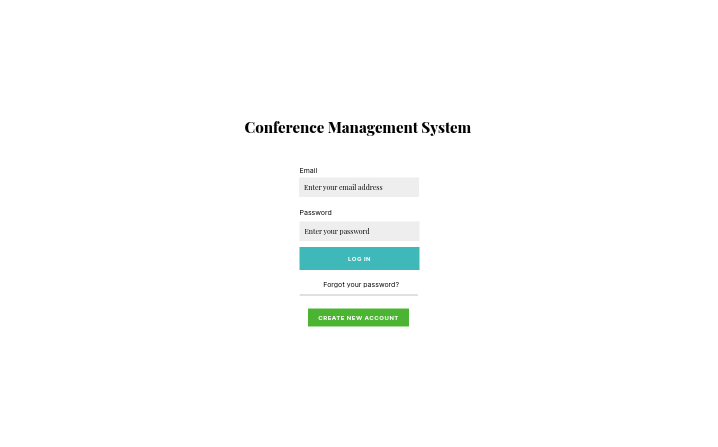
\includegraphics[keepaspectratio,width=18cm,height=12cm]{UI-Wireframes/login_screen.png}}
\caption{Login Screen}
\end{figure}


\newpage
\section{Profile Creation Page:}
\begin{figure}[h!]
\centering
 \fbox{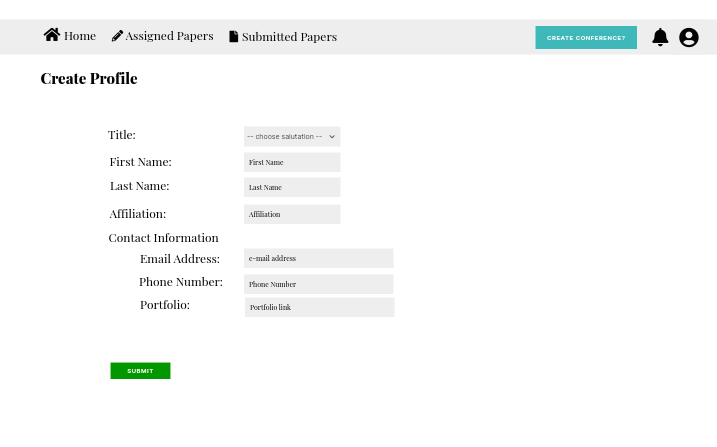
\includegraphics[keepaspectratio,width=18cm,height=12cm]{UI-Wireframes/profile_creation.png}}
\caption{Profile Creation Page}
\end{figure}


\newpage
\section{Profile Page:}
\begin{figure}[h!]
\centering
 \fbox{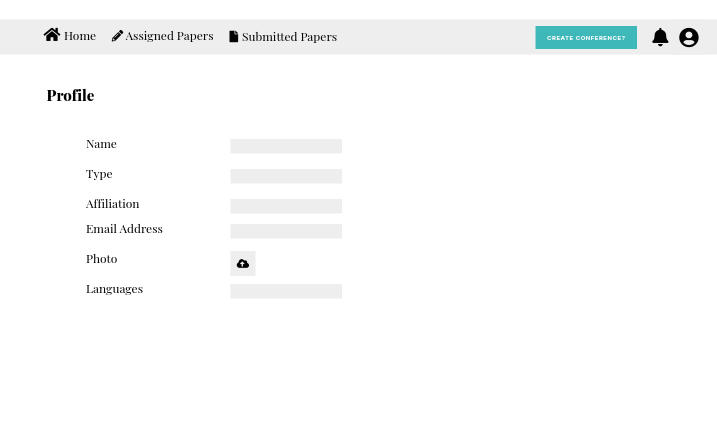
\includegraphics[keepaspectratio,width=18cm,height=12cm]{UI-Wireframes/profile_page.png}}
\caption{Profile Page}
\end{figure}


\newpage
\section{Main Page:}

\begin{figure}[h!]
\centering
 \fbox{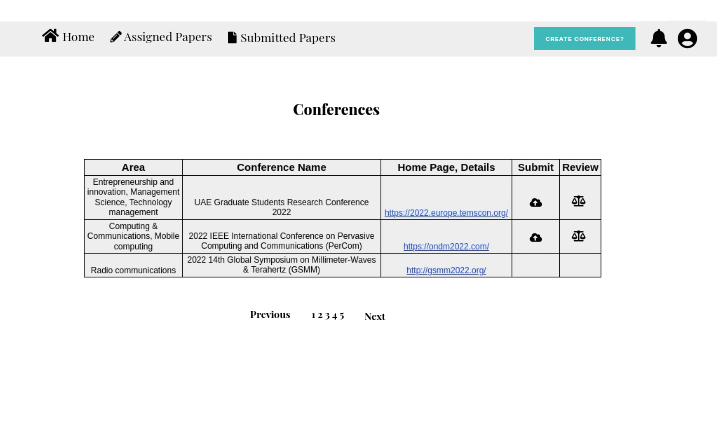
\includegraphics[keepaspectratio,width=18cm,height=12cm]{UI-Wireframes/main_page.png}}
\caption{Main Page}
\end{figure}



\newpage
\section{Conference Creation Page:}
\begin{figure}[h!]
\centering
 \fbox{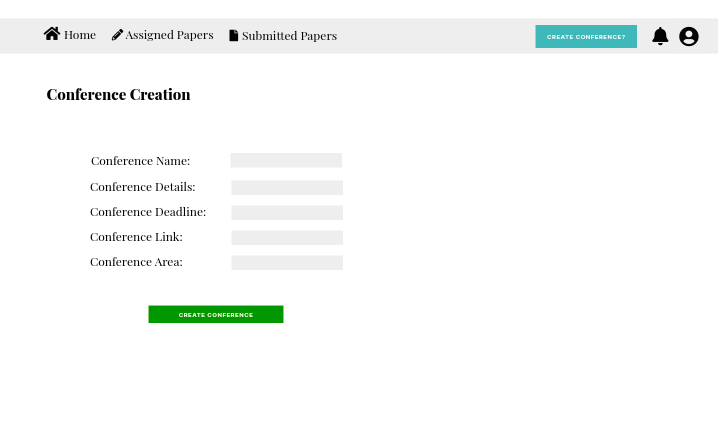
\includegraphics[keepaspectratio,width=18cm,height=12cm]{UI-Wireframes/create_conference_page.png}}
\caption{Conference Creation Page}
\end{figure}



\newpage
\section{Paper Submission Page:}
\begin{figure}[h!]
\centering
 \fbox{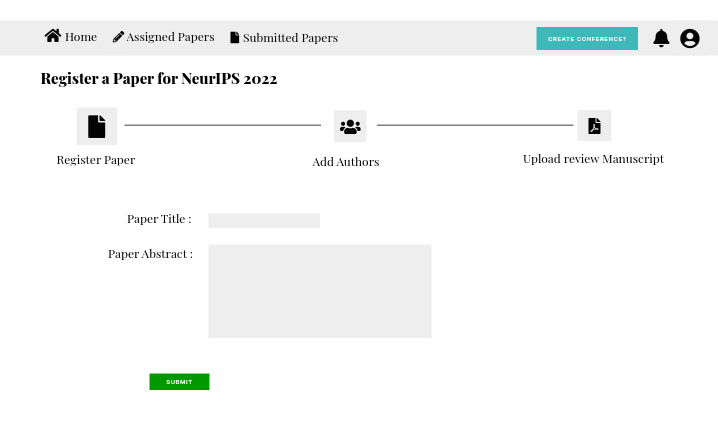
\includegraphics[keepaspectratio,width=18cm,height=12cm]{UI-Wireframes/submit_paper.png}}
\caption{Paper Submission Page}
\end{figure}



\newpage
\section{Reviewer Registration Page:}
\begin{figure}[h!]
\centering
 \fbox{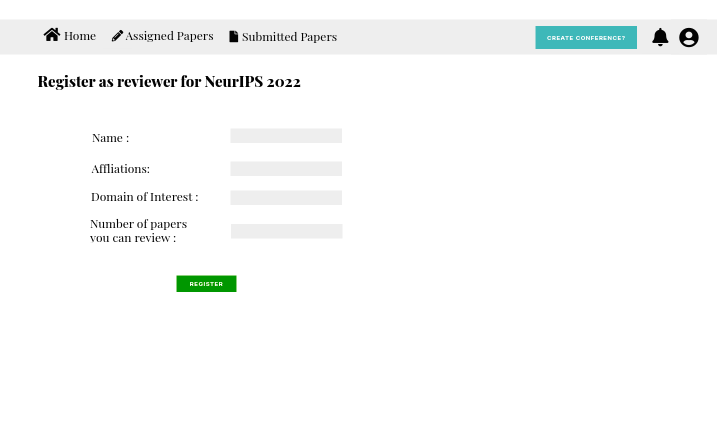
\includegraphics[keepaspectratio,width=18cm,height=12cm]{UI-Wireframes/reviewer_registration.png}}
\caption{Reviewer Registration Page}
\end{figure}


\newpage
\section{Assigned Papers Page:}
\begin{figure}[h!]
\centering
 \fbox{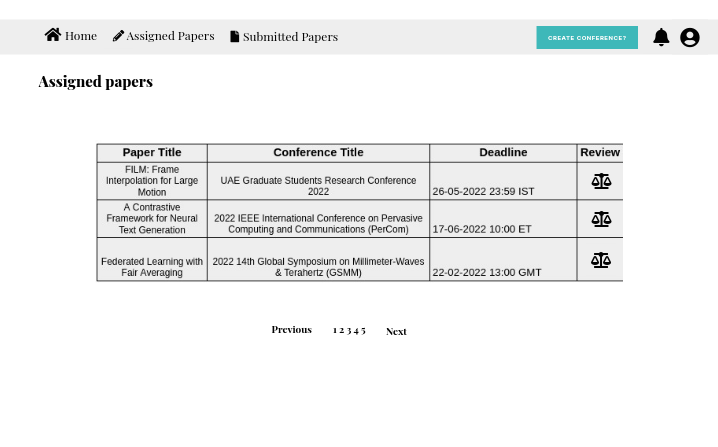
\includegraphics[keepaspectratio,width=18cm,height=12cm]{UI-Wireframes/assigned_papers.png}}
\caption{Assigned Papers Page}
\end{figure}



\newpage
\section{Submitted Papers Page:}
\begin{figure}[h!]
\centering
 \fbox{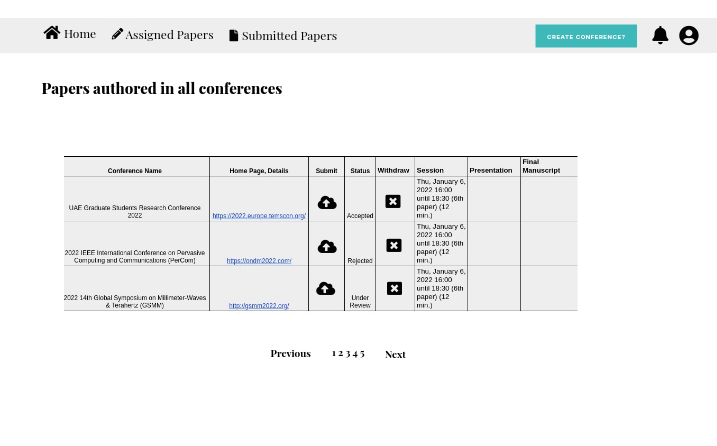
\includegraphics[keepaspectratio,width=18cm,height=12cm]{UI-Wireframes/submitted_papers.png}}
\caption{Submitted Papers Page}
\end{figure}


\newpage
\section{Help Page:}
\begin{figure}[h!]
\centering
 \fbox{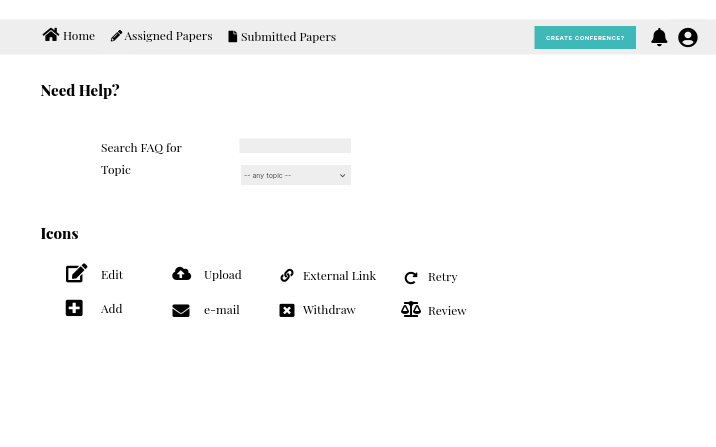
\includegraphics[keepaspectratio,width=18cm,height=12cm]{UI-Wireframes/help_page.png}}
\caption{Help Page}
\end{figure}



\end{document}